\documentclass[12pt]{article}
\usepackage{amsmath}
\usepackage{graphicx}
\usepackage{hyperref}
\usepackage[latin1]{inputenc}
\title{Rangkuman Basis Data Pertemuan 2 Dan Pembuatan Absensi Mahasiwa}
\date{}
\begin{document}
\begin{titlepage}
\maketitle
\thispagestyle{empty}

\vspace{0.5cm}
\begin{center}

\includegraphics[width=5cm, height=5cm]{poltekpos.png}
\end{center}
\vspace{0.5cm}
\begin{center}
Diajukan untuk memenuhi tugas mata kuliah Basis Data\\
\vspace{12px}
Dosen Pengampu:\\
Syafrial Fachri Pane, ST., MTI., EBDP.
\vspace{12px}

Oleh:\\
Muhammad Rafly Fachrian Al Bantani\\
1194058
\vspace{14px}

\textbf{PROGRAM DIPLOMA IV TEKNIK INFORMATIKA}\\
\textbf{POLITEKNIK POS INDONESIA\\}\textbf{BANDUNG}\\
\textbf{2020}
\end{center}
\end{titlepage}


\newpage
\maketitle

Basis adalah Tempat/Gudang.

Data adalah Nilai Value yang merepresentasikan deskripsi dari suatu objek atau kejadian

Objek/Kejadian direkam disimpan berupa bukti contohnya struk belanja saat belanja (Data yang mempunyai rekamannya itu Valid)

Data itu sangat pentik maka teknologi pun bersumber dari data, data dijadikan untuk ekonomi dan masih banyak lainnya.

Relasi menghubungkan menjadi satu kesatuan dan key lah yang menjadikan relasi semakin erat

Database Mempunyai 4 key/kunci yang mendati identitas suatu data 
\begin{itemize}
  \item Primary Key yang bersifat Unik dan juga key untuk mewakili suatu data
  \item Foreign key adalah kunci tamu yang dimana dia adalah primary key dari domennya dan juga sebagai penghubung antar entity
  \item Candidate key adalah kunci yang mengidentifikasi dengan unik
  \item Super key adalah kunci yang tidak dipakai sebagai primary key
        \hspace*{3cm}
        
        Database dibagi menjadi dua yaitu :
        \item SQL yaitu database yang mengutamakan struktur, dengan struktur yang tersusun jadi lebih menguntungkan disebagian kondisi contohnya untuk menyimpan data penduduk yang harus terstruktur.
        \item NoSQL yaitu database yang mengutamakan kecepatan seperti contohnya penyimpanan data pada instagram yang langsung tersimpan tidak terstruktur yang memudahkan mengambil foto dengan cepatnya.
\end{itemize}

Basis data ada yang relasional datanya harus dikelompokan dan direlasikan bertujuan untuk memudahkan, mengurangi redundansi dan tidak ada batasan pada pencarian data.

\vspace{5cm}
\textbf{Tugas Membuat Aplikasi Absensi}

\vspace{1cm}
Pada tugas kali ini membuat CDM dan PDM dari absensi mahasiswa. 

\begin{enumerate}
 \item CDM


berikut adalah gambar dari CDM yang telah saya buat.
\begin{center}
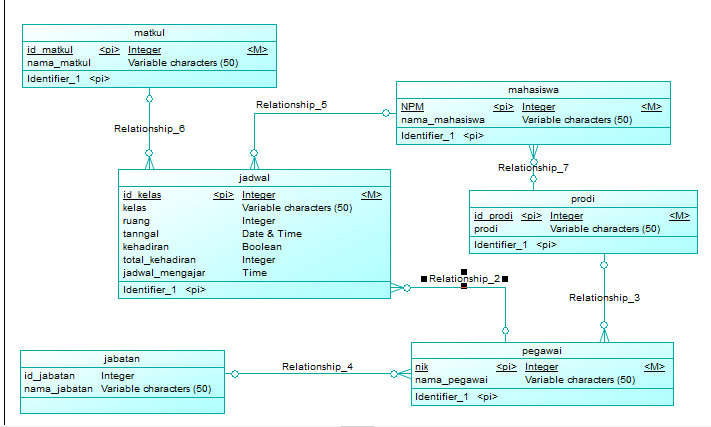
\includegraphics[width=10cm, height=10cm]{CDM.png}
\end{center}

Pada Gambar diatas dapat dijelaskan bahwa tabel Jadwal Matkul adalah master data yang berelasi dengan entities yang lain.
\begin{itemize}
  \item Tabel Program studi memiliki 2 atribut yaitu Kode program studi sebagai primary keynya dan nama program studi, tabel ini berelasi dengan tabel mahasiswa
  \item Tabel Mahasiswa tersiri dari 3 atribut yaitu NPM sebagai primary keynya, nama mahasiswa dan nama program studi yang bisa diambil dari tabel prgram studi
  \item Tabel Matkul berisikan 2 atribut yaitu kode matkul yang menjadi primary key dan nama matkul. tabel ini langsung berelasi dengan master data yaitu tabel jadwal matkul
  \item Tabel Jabatan berisikan 2 atribut yaitu kode jabatan yang merupakan primary key dan nama jabatan yang berelasi dengan tabel pegawai
  \item Tabel Pegawai memiliki 3 atribut yaitu NIK yang merupakan primary key, nama pegawai dan nama jabatan yang langsung bisa diambil dari tabel jabatan. tabel pegawai berelasi dengan jadwal matkul yang merupakan master data.
  
  NOTED : Primary key yang sudah berelasi maka menjadi foreign key pada antities yang berelasi tersebut.
        \hspace*{3cm}
\end{itemize} 
        

 \item PDM
\end{enumerate} 
        
berikut adalah gambar dari PDM yang telah saya buat dari hasil generate dari CDM ke PDM

\begin{center}
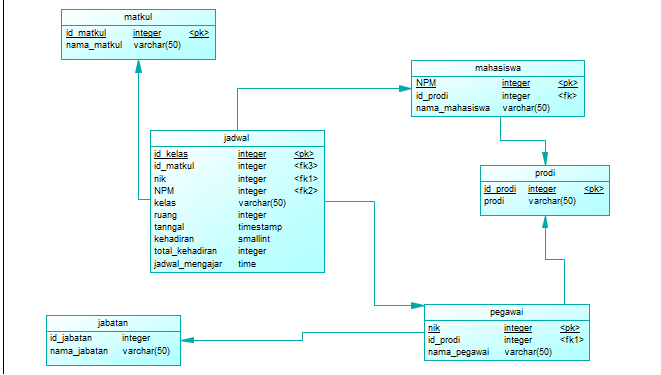
\includegraphics[width=10cm, height=10cm]{PDM.png}
\end{center}
        
Pada Gambar diatas dapat dijelaskan bahwa tabel Jadwal Matkul adalah master data yang berelasi dengan entities yang lain.
\begin{itemize}
  \item Tabel Program studi memiliki 2 atribut yaitu Kode program studi sebagai primary keynya dan nama program studi, tabel ini berelasi dengan tabel mahasiswa
  \item Tabel Mahasiswa tersiri dari 3 atribut yaitu NPM sebagai primary keynya, nama mahasiswa dan nama program studi yang bisa diambil dari tabel prgram studi
  \item Tabel Matkul berisikan 2 atribut yaitu kode matkul yang menjadi primary key dan nama matkul. tabel ini langsung berelasi dengan master data yaitu tabel jadwal matkul
  \item Tabel Jabatan berisikan 2 atribut yaitu kode jabatan yang merupakan primary key dan nama jabatan yang berelasi dengan tabel pegawai
  \item Tabel Pegawai memiliki 3 atribut yaitu NIK yang merupakan primary key, nama pegawai dan nama jabatan yang langsung bisa diambil dari tabel jabatan. tabel pegawai berelasi dengan jadwal matkul yang merupakan master data.
  
  NOTED : Primary key yang sudah berelasi maka menjadi foreign key pada antities yang berelasi tersebut.
        \hspace*{3cm}

Secara keseluruhan isi CDM dan PDM terlihat sama tapi mempunyai perbedaan yaitu kalau CDM dia hanya tabel yang berdiri sendiri kalau PDM akan terlihat foreign keynya yang mana serta primarynya 

Tabel yang mempunyai relasi foreign key akan terlihat ada penambahan atribut dari entities lainnya

Contoh kode matkul pada CDM tidak ada tapi pada PDM ada.

Dan juga bila pada PDM relasinya terlihat seperti panah yang mengarah antar entities.

PDM juga adalah bentuk fisik dari database itu sendiri jadi bisa langsung di masukan dan akan langsung menjadi database.
\end{itemize}
\end{document}
